\documentclass[18pt]{beamer}
\usepackage[utf8]{inputenc} % for the umlauts
\usepackage{subfigure}

\beamertemplatenavigationsymbolsempty
%% SLIDE FORMAT

% use 'beamerthemekit' for standard 4:3 ratio
% for widescreen slides (16:9), use 'beamerthemekitwide'

\usepackage{templates/beamerthemekit}
% \usepackage{templates/beamerthemekitwide}

\setcounter{tocdepth}{1}

%% TITLE PICTURE

% if a custom picture is to be used on the title page, copy it into the 'logos'
% directory, in the line below, replace 'mypicture' with the 
% filename (without extension) and uncomment the following line
% (picture proportions: 63 : 20 for standard, 169 : 40 for wide
% *.eps format if you use latex+dvips+ps2pdf, 
% *.jpg/*.png/*.pdf if you use pdflatex)

%\titleimage{mypicture}

%% TikZ INTEGRATION

% use these packages for PCM symbols and UML classes
% \usepackage{templates/tikzkit}
% \usepackage{templates/tikzuml}

% the presentation starts here

\usepackage{mathabx}
\usepackage{picture}
\usepackage[absolute,overlay]{textpos}
%\usepackage[texcoord,grid,gridunit=mm,gridcolor=red, subgridcolor=green]{eso-pic}
\setbeamercovered{invisible}
\setbeamertemplate{caption}{\raggedright\insertcaption\par}

\title[SWT1]{Softwaretechnik 1 - 3. Tutorium}
\subtitle{Tutorium 03}
\author{Felix Bachmann}
\date{05.06.2018}

\institute{KIT - Institut für Programmstrukturen und Datenorganisation (IPD)}

% Bibliography

\usepackage[citestyle=authoryear,bibstyle=numeric,hyperref,backend=biber]{biblatex}
\addbibresource{templates/example.bib}
\bibhang1em

\begin{document}

% change the following line to "ngerman" for German style date and logos
\selectlanguage{ngerman}

%title page
\begin{frame}
\titlepage
\end{frame}

\section{Orga}
	\subsection{Feedback 3. Übungsblatt}
	\begin{frame}
		\frametitle{3. Übungsblatt Statistik}
		%TODO
		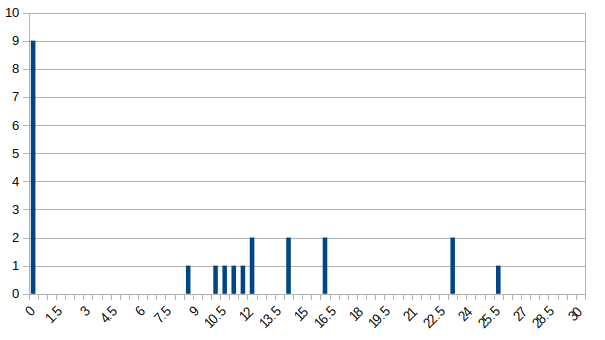
\includegraphics[scale=0.7]{./pics/tut3/statistics-ub3.png}
		\linebreak \centering $\diameter$ 11,56 bzw. 16,32 von 28+1
	\end{frame}
	
	\subsection{3. Übungsblatt - Fehler (Allgemein)}
	\begin{frame}
		\frametitle{Häufige Fehler}
		%TODO
		\begin{block}{Allgemein}
			\begin{itemize}
				\item verspätete Abgaben bekomme ich erst beim jeweils nächsten Tutorentreffen	
				\linebreak $\implies$ Rückgabe dauert länger; gibt keine Punkte, nur grobe Korrektur
			\end{itemize}
		\end{block}
	\end{frame}
	
	\subsection{3. Übungsblatt - Fehler}
	\begin{frame}
		\frametitle{Häufige Fehler}
		\begin{block}{Aufgabe 1 (Plug-In-Architektur: PluginManager + JmjrstPlugin)}
			\begin{itemize}
				\item Plugins anhand \textbf{Klassen}namen vergleichen, nicht getName() \pause
				\item Strings auslagern (Konstanten oder Datei) \pause
				\item PluginManager gibt euch Iterable $\implies$ nutzt Iterator
				\begin{itemize}
					\item kein Casten, Kopieren in Liste \pause
				\end{itemize}
 				\item orientiert euch nicht am JMJRST-Stil
			\end{itemize}
		\end{block}
	\end{frame}

	\begin{frame}
		\frametitle{Häufige Fehler}
		\begin{block}{Aufgabe 2 (Plug-In)}
			\begin{itemize}
				\item Prüfen auf *.png/*.jpg sollte case insensitive sein \pause
				\item Anm.: MetainfServices tut manchmal nicht richtig (oft hilft \texttt{mvn clean package}) \pause
			\end{itemize}
		\end{block}
		\begin{block}{Aufgabe 3 (iMage-Bundle)}
			\begin{itemize}
				\item keine :D
			\end{itemize}
		\end{block}
	\end{frame}

	\begin{frame}
		\frametitle{Häufige Fehler}
		\begin{block}{Aufgabe 4 (Aktivitätsdiagramm)}
			%TODO
			\begin{itemize}
				\pause 
				\item denkt an die Rauten! \pause
				\item $\lbrack$Bedingung$\rbrack$ \pause
				\item verschachtelte Aktivitäten $\implies$ irgendwo passender Kasten dazu
			\end{itemize}
		\end{block}
	\end{frame}

	\begin{frame}
		\frametitle{Häufige Fehler}
		\begin{block}{Aufgabe 5 (Zustandsdiagramm)}
			%TODO
		\end{block}
	\end{frame}

	\begin{frame}
		\frametitle{Häufige Fehler}
		\begin{block}{Aufgabe 6 (Sequenzdiagramm)}
			%TODO
			\begin{itemize}
				\pause 
				\item bzgl. Konstruktor sind VL-Folien etwas blöd \pause
				\item asynchron vs. synchron (Pfeilspitzen sind wichtig!) \pause
				\item nicht statische Instanzen unterstreichen \pause
				\item Instanz-Kästen erst dann hinzeichnen, wenn Instanz auch existiert
			\end{itemize}
		\end{block}
		\begin{block}{Aufgabe 7 (Testen mit Nachahmungen)}
			%TODO
		\end{block}
	\end{frame}



\section{Motivation}
	\subsection{Kontext}
		\begin{frame}
			\frametitle{Wo sind wir?}
			\begin{itemize}
				\item die ersten 2 Phasen des Wasserfallmodells sind geschafft
				\pause
				\linebreak $\implies$ Welche waren das nochmal? \pause Planung, Definition!
				\pause
				\linebreak $\implies$ Dokumente? \pause Lastenheft, Pflichtenheft (+ andere\dots)
				\pause
				\item  jetzt: Entwurf!
			\end{itemize}
		\end{frame}
	
		\begin{frame}
			\frametitle{Wozu Entwurf?}
			\centering
			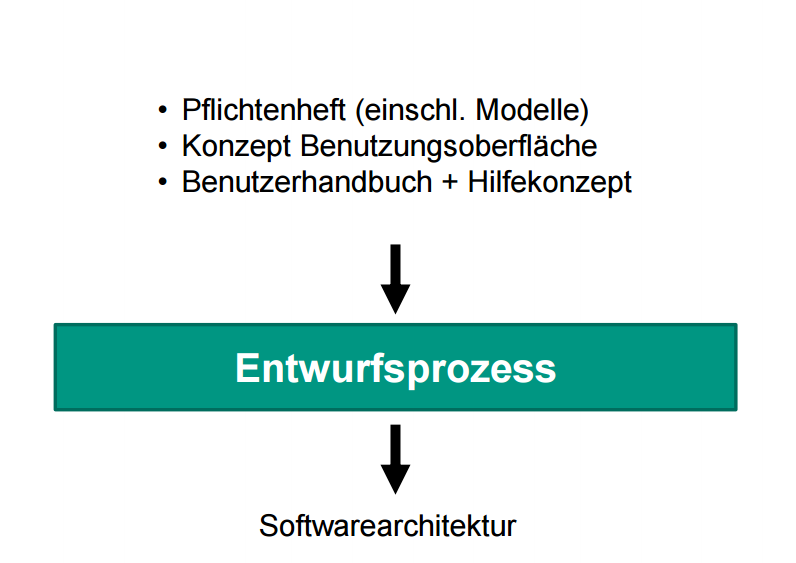
\includegraphics[scale=0.4]{./pics/tut3/design.png} \linebreak
			Softwarearchitektur ist Grundlage für Implementierung!
		\end{frame}
	
		\begin{frame}
			\frametitle{Abgrenzung Definition vs. Entwurf}
			\begin{itemize}
				\item Definition: \textbf{Was} ist zu implementieren?
				\pause
				\item Entwurf: \textbf{Wie} ist das System zu implementieren?
			\end{itemize}
		\end{frame}
	
\section{Entwurfsmuster}
	\subsection{Grundlagen}
	
	\begin{frame}
		\frametitle{Empfehlenswerte Literatur (wirklich!)}
		knapp 700 Seiten \linebreak $\implies$ als interaktives Nachschlagewerk, falls man bestimmte Muster nicht versteht \linebreak
		\centering
		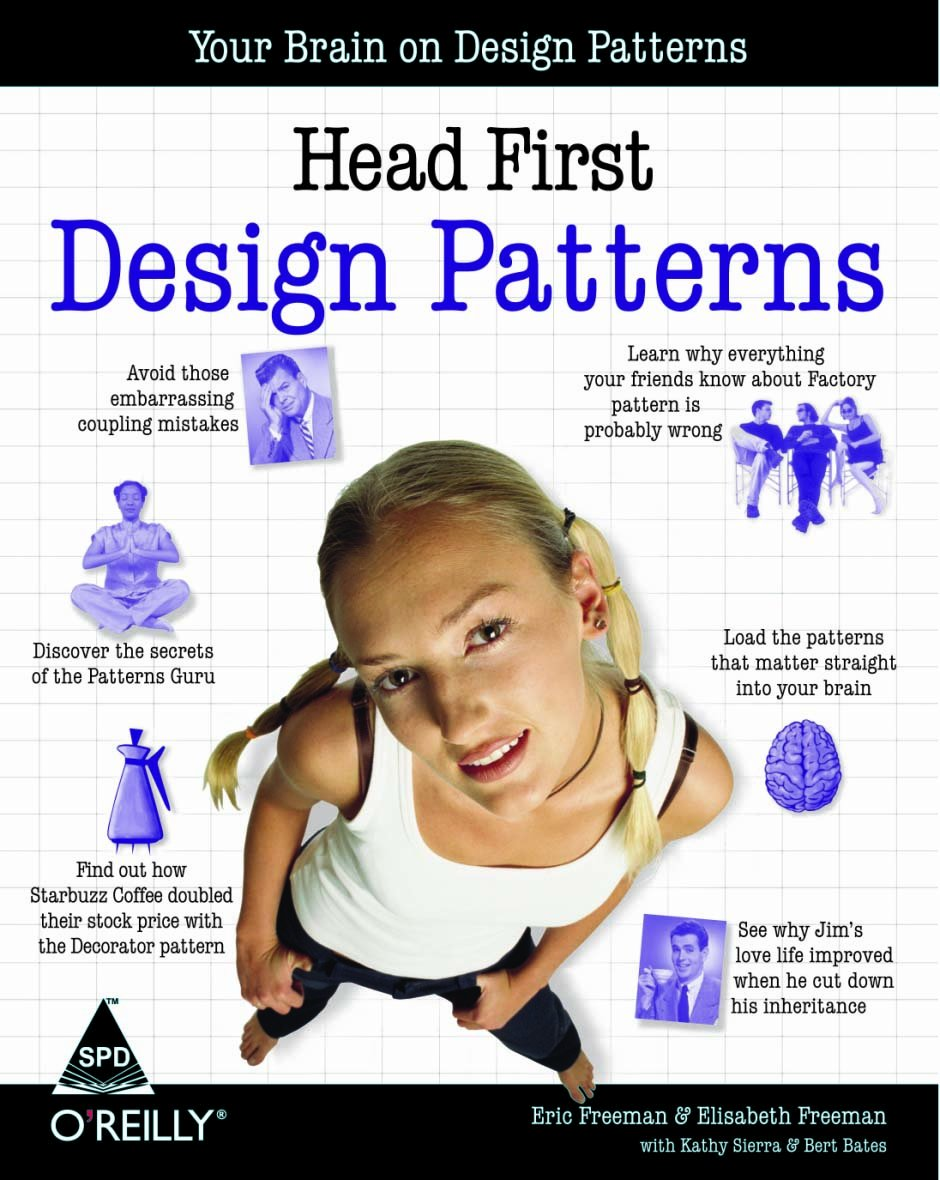
\includegraphics[scale=0.15]{./pics/tut3/literature.jpg}
	\end{frame}
		
	\begin{frame}
		\frametitle{Was sind Entwurfsmuster?}
		\begin{block}{Entwurfsmuster}
			Ein Software-Entwurfsmuster beschreibt eine
			Familie von Lösungen für ein Software-Entwurfsproblem.
		\end{block}
		\pause
		\begin{itemize}
			\item schematische Klassendiagramme zur Lösung von häufig auftretenden Problemen \pause
			\item Wiederverwendung von Entwurfswissen $\implies$ Rad nicht neu erfinden!
		\end{itemize}
		\pause
		\centering
		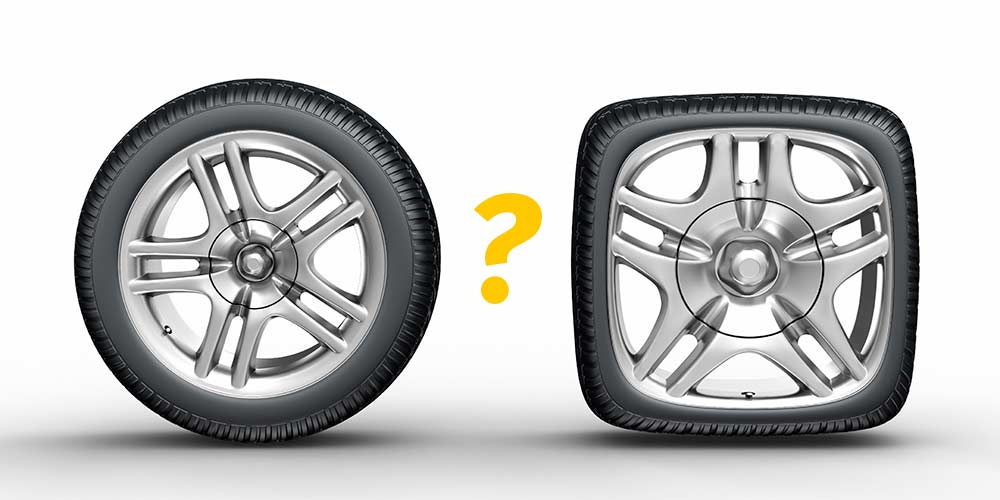
\includegraphics[scale=0.2]{./pics/tut3/new-wheel.jpg}
	\end{frame}

	\begin{frame}
		\frametitle{Wozu Entwurfsmuster?}
		\begin{itemize}
			\item erleichtern Kommunikation \pause
			\item erleichtern "'gute"' Entwürfe und das Schreiben von wartbarem/erweiterbarem Code
		\end{itemize}
\end{frame}
	
	\begin{frame}
		\frametitle{Geheimnisprinzip}
		\begin{block}{Geheimnis- / 
				Kapselungsprinzip}
			Jedes Modul verbirgt eine wichtige
			Entwurfsentscheidung hinter einer
			wohldefinierten Schnittstelle, die sich bei einer
			Änderung der Entscheidung nicht mit ändert.
		\end{block}
		\pause
		\begin{alertblock}{Warum eigentlich?}
			lokale Änderungen sollen sich nicht auf andere Teile auswirken 
			\linebreak $\implies$ weniger Fehler und Arbeit
		\end{alertblock}
		Beispiel? \pause $\implies$ private Attribute mit get()- und set()-Methoden
	\end{frame}

	\begin{frame}
		\frametitle{Vorgriff: Entwurfsmuster Strategie}
		\begin{itemize}
			\item Ziel: Algorithmen kapseln, austauschbar machen
			\item wird in vielen Entwurfsmustern verwendet
		\end{itemize}
		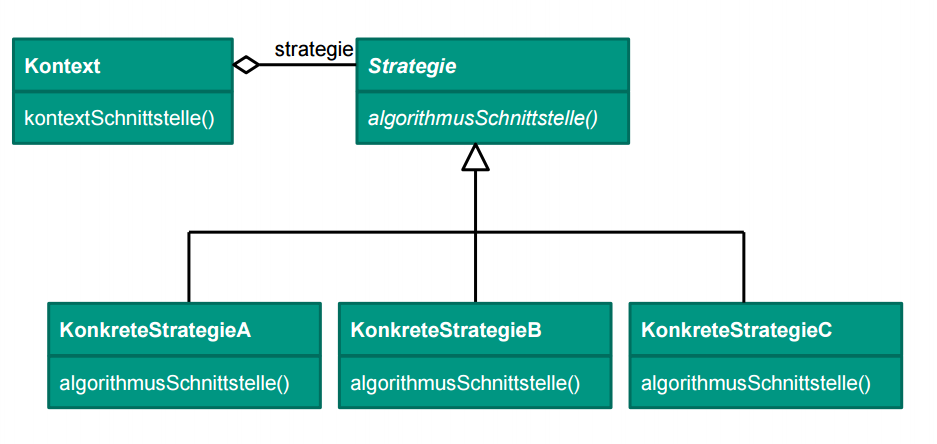
\includegraphics[scale=0.5]{./pics/tut3/strat.png}
	\end{frame}

	\begin{frame}
		\frametitle{Quiz (Ankreuzaufgaben aus Klausuren)}
		Wahr oder falsch?
		\begin{itemize}
			\item Das Entwurfsmuster Strategie bietet die Möglichkeit, eine Klasse mit einer von mehreren möglichen Verhaltensweisen zu konfigurieren. \pause \colorbox{green}{wahr} \pause
			\item Das Strategiemuster erfüllt das Geheimnisprinzip, indem es Datenstrukturen, die in einer konkreten Strategie enthalten sind, vor dem Klienten verbirgt. \pause \colorbox{green}{wahr} \pause
			\item Das Muster Strategie kapselt austauschbares Verhalten und verwendet Delegierung, um zu entscheiden, welches Verhalten verwendet wird. \pause \colorbox{green}{wahr} \pause 
			\item Das Hinzufügen einer neuen konkreten Strategie erfordert keine Änderung existierender konkreter Strategien. \pause \colorbox{green}{wahr}
		\end{itemize}
\end{frame}

	\begin{frame}
		\frametitle{Kategorien der Entwurfsmuster}
		\begin{itemize}
			\item \textbf{Entkopplungs-Muster}
				\begin{itemize}
					\item \textbf{Adapter}
					\item \textbf{Beobachter}
					\item \textbf{Iterator}
					\item \textbf{Stellvertreter}
					\item \textbf{Vermittler}
					\item Brücke
				\end{itemize}
			\item Varianten-Muster
			\item Zustandshandhabungs-Muster
			\item Steuerungs-Muster
			\item Bequemlichkeits-Muster
		\end{itemize}
	\end{frame}

	\begin{frame}
		\frametitle{Entkopplungs-Muster}
		\begin{itemize}
			\item übergeordnetes Ziel: System in Teile aufspalten, die unabhängig voneinander sind
			\linebreak $\implies$ Teile austauschbar bzw. veränderbar
	\end{itemize}
	\end{frame}

\section{Adapter}
	\subsection{Adapter}
	\begin{frame}
		\frametitle{Adapter}
		\begin{block}{Problem}
			\begin{itemize}
				\item Klassen mit inkompatiblen Schnittstellen, die wir aber zusammen benutzen wollen 
				\item Schnittstellen nicht änderbar (z.B. externe Bibliotheken)
			\end{itemize}
		\end{block}
		\pause
		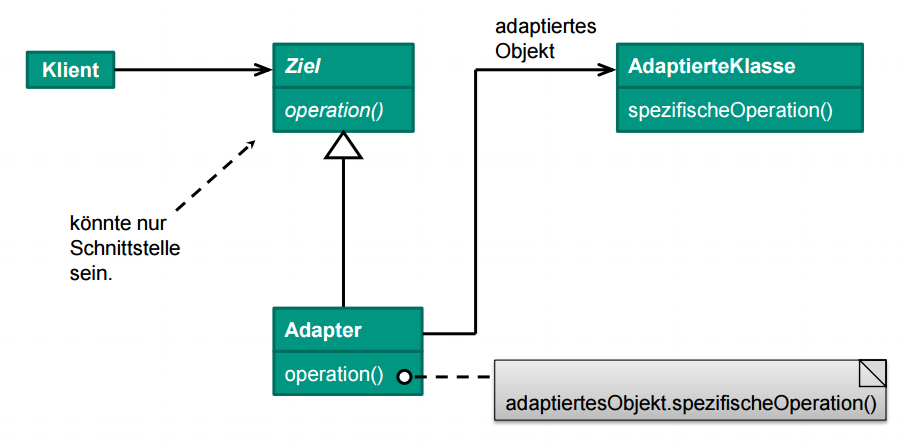
\includegraphics[scale=0.45]{./pics/tut3/adap-obj.png}
	\end{frame}

	\begin{frame}
		\frametitle{Adapter (Objektadapter)}
		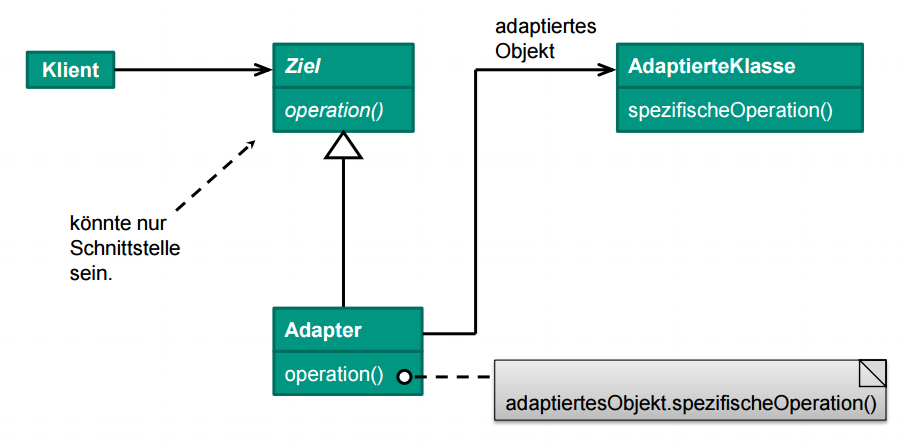
\includegraphics[scale=0.45]{./pics/tut3/adap-obj.png}
		\begin{block}{Wir sind bei Entkopplung-Mustern, Preisfrage:}
			Wo ist hier die Entkopplung?
			\pause
			\linebreak der Klient ist von der adaptierten Klasse entkoppelt $\implies$ austauschbar
		\end{block}
	\end{frame}

	\begin{frame}
		\frametitle{Adapter - Alternative (Klassenadapter)}
		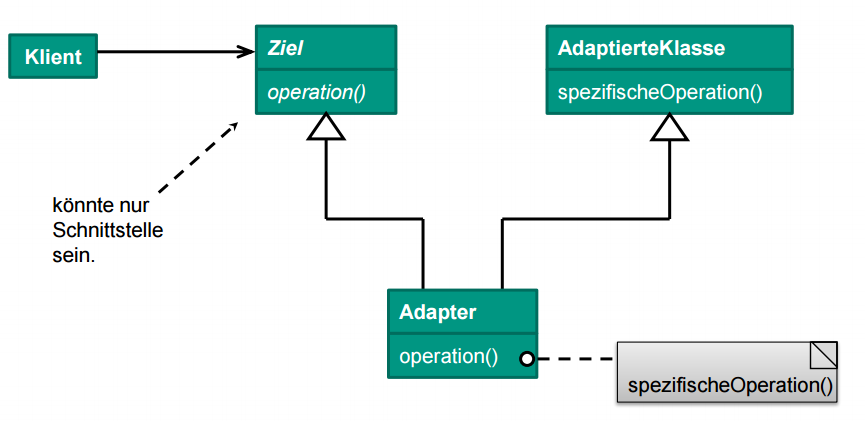
\includegraphics[scale=0.45]{./pics/tut3/adap-cl.png} \linebreak \pause
		Was für ein Problem bekommt ihr, wenn ihr das auf einem ÜB implementieren müsst? \pause \linebreak
		$\implies$ keine Mehrfachvererbung in Java!
	\end{frame}

\section{Beobachter}
	\subsection{Beobachter}
	\begin{frame}{Beobachter/Observer: abstrakt}
		\begin{block}{Problem}
			\begin{itemize}
				\item ein Subjekt, viele Beobachter
				\item Subjekt ändert Zustand $\implies$ Beobachter machen "'irgendwas"
			\end{itemize}		
		\end{block}
	\end{frame}

	\begin{frame}{}
		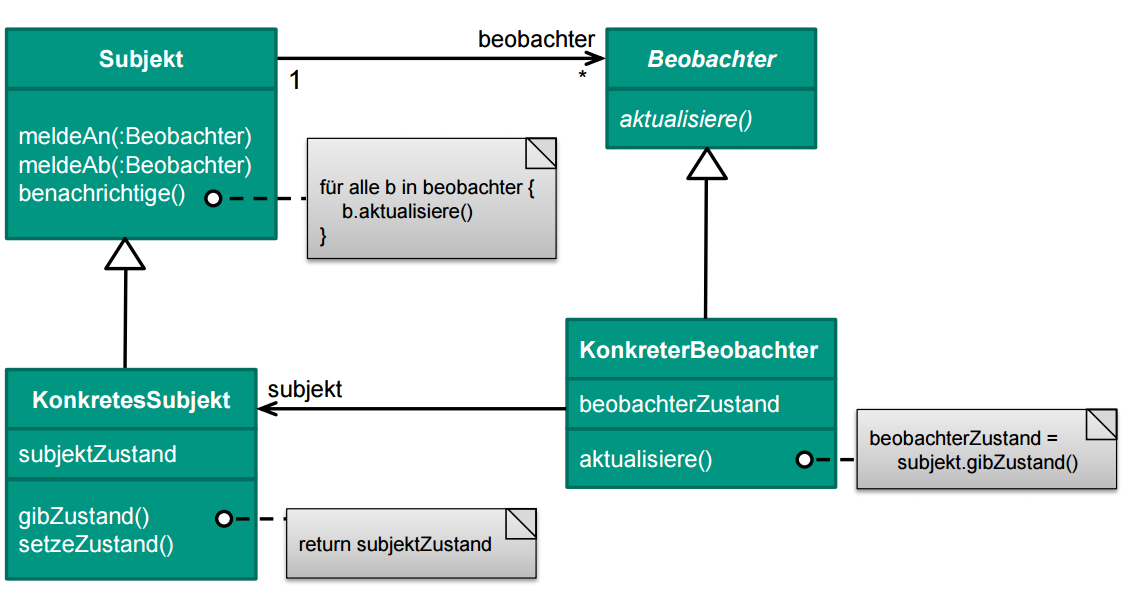
\includegraphics[keepaspectratio, width=\textwidth, height=\textheight]{pics/tut3/obs.png}
		\pause
		\begin{block}{Entkopplung?}
		\begin{itemize}
			\pause 
			\item jeder Beobachter definiert, was bei Benachrichtigung passiert, Subjekt kriegt davon nichts mit \pause
			\item zur Laufzeit änderbar: Anzahl der Beobachter
		\end{itemize}
		\end{block}
	\end{frame}

	\begin{frame}{Beobachter/Observer: am Beispiel}
		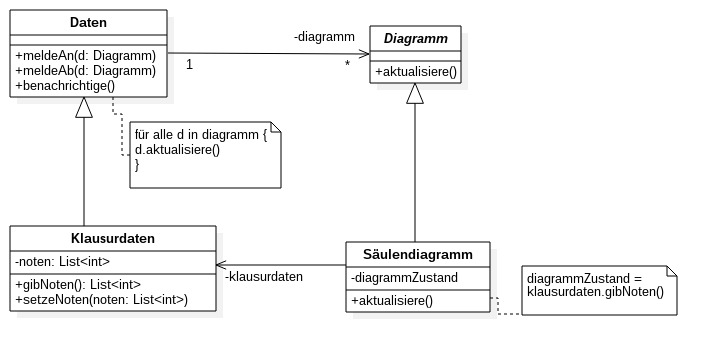
\includegraphics[keepaspectratio, width=\textwidth, height=\textheight]{pics/tut3/observer_example.jpg}
	\end{frame}

\section{Iterator}
	\subsection{Iterator}
	\begin{frame}
		\frametitle{Iterator}
		\begin{block}{Problem}
			\begin{itemize}
				\item wollen über Datenstruktur iterieren + Operationen ausführen \linebreak $\implies$ Hinzufügen, Löschen\dots \pause
				\item das Ganze ohne Kentniss des internen Aufbaus der Datenstruktur 
			\end{itemize}
		\end{block}
		\pause
		\centering
		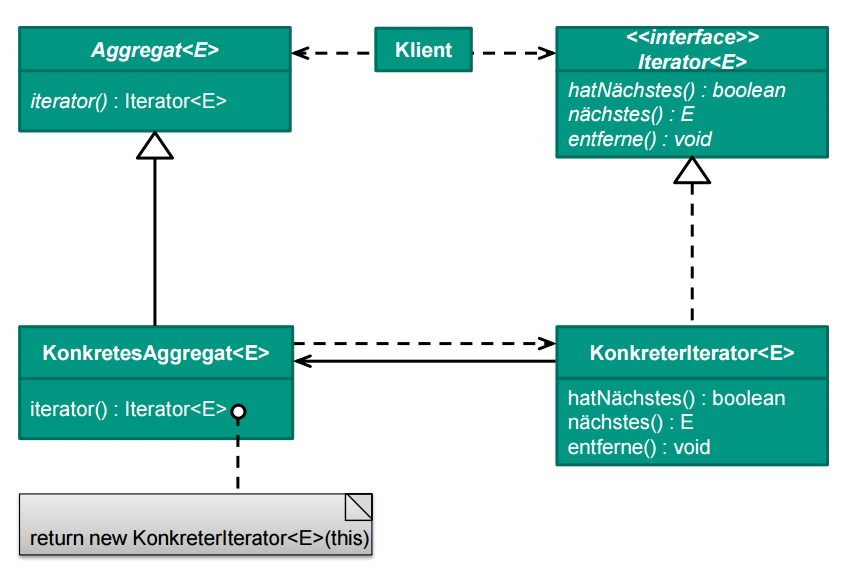
\includegraphics[scale=0.35]{./pics/tut3/iter.png}
	\end{frame}

	\begin{frame}
		\frametitle{Iterator}
		\centering
		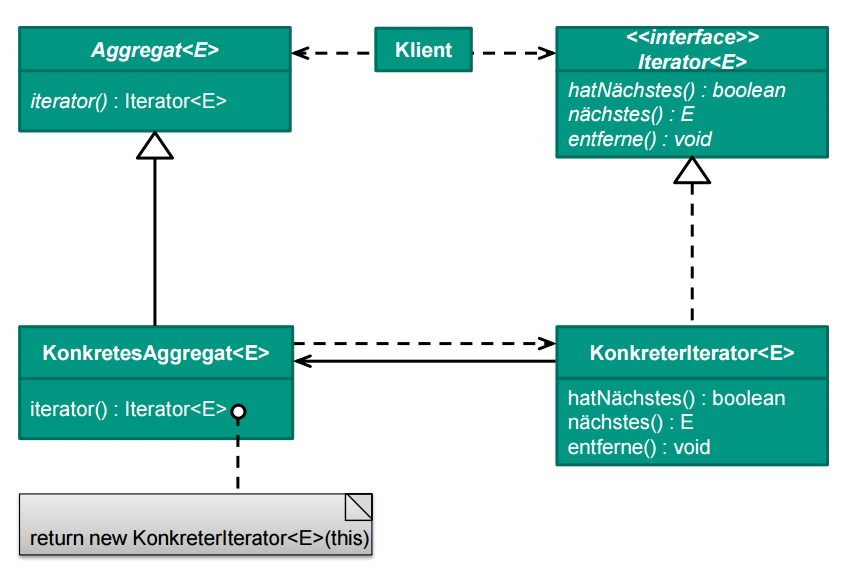
\includegraphics[scale=0.35]{./pics/tut3/iter.png}
		\begin{block}{Entkopplung?}
			\begin{itemize}
				\pause 
				\item Klient benutzt nur Methoden der Schnittstelle auf dem konkreten Iterator \linebreak $\implies$ Implementierung austauschbar
			\end{itemize}
		\end{block}
	\end{frame}
	
	\begin{frame}
		\frametitle{Iterator}
		\centering
		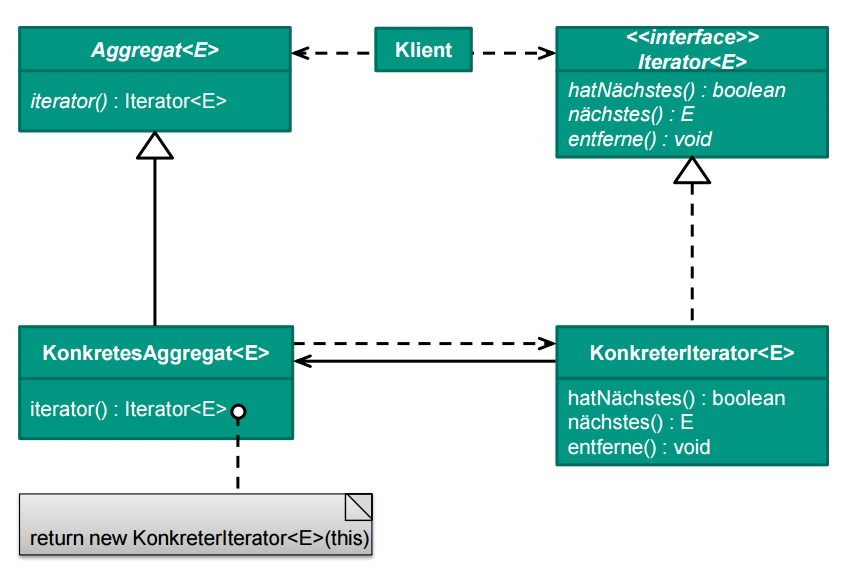
\includegraphics[scale=0.35]{./pics/tut3/iter.png}
		\linebreak Beispiel in Java: list.iterator();
	\end{frame}

	\begin{frame}
		\frametitle{Quiz (Ankreuzaufgaben aus Klausuren)}
		Wahr oder falsch?
		\begin{itemize}
			\item Klienten können mithilfe des Iterator-Musters Sammlungen von Objekten und einzelne Objekte auf die gleiche Weise behandeln. \pause \colorbox{red}{falsch} \pause
			\item Das Entwurfsmuster Iterator ist den Variantenmustern zuzuordnen. \pause \colorbox{red}{falsch} 
		\end{itemize}
	\end{frame}

\section{Stellvertreter}
	\subsection{Stellvertreter}
	\begin{frame}
		\frametitle{Stellvertreter}
		\begin{block}{Problem}
			\begin{itemize}
				\item wollen Zugriff auf ein Objekt kontrollieren, ohne seine Klasse zu ändern \linebreak \pause $\implies$ Stellvertreter macht Zugriffskontrolle
			\end{itemize}
		\end{block}
		\pause
		\centering
		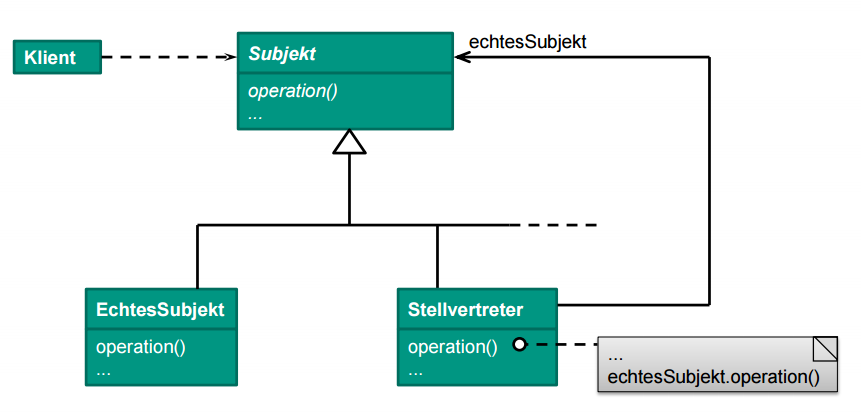
\includegraphics[scale=0.4]{./pics/tut3/prox.png}
	\end{frame}

	\begin{frame}
		\frametitle{Stellvertreter}
		\centering
		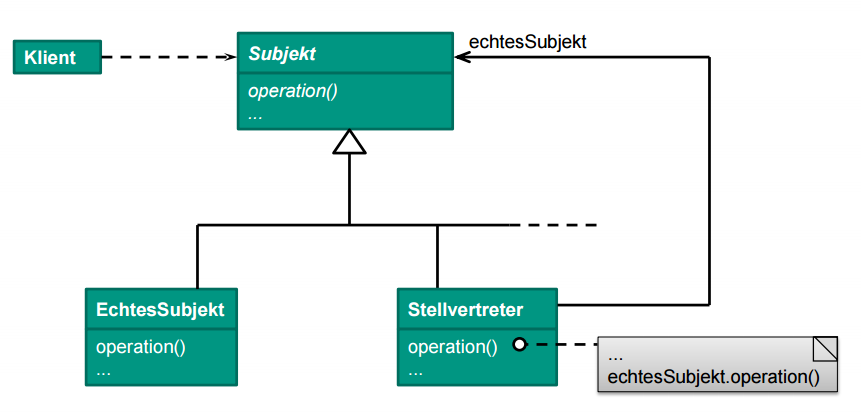
\includegraphics[scale=0.4]{./pics/tut3/prox.png}
		\begin{block}{Entkopplung?}
			\begin{itemize}
				\pause 
				\item Klient hat keinen direkten Zugriff auf das echte Subjekt
			\end{itemize}
		\end{block}
	\end{frame}

\section{Vermittler}
	\subsection{Vermittler}
		\begin{frame}
		\frametitle{Vermittler}
		\begin{block}{Problem}
			\begin{itemize}
				\item mehrere voneinander abhängige Objekte \linebreak \pause $\implies$ Zustände der Objekte von anderen Zuständen abhängig
			\end{itemize}
		\end{block}
		\pause
		\centering
		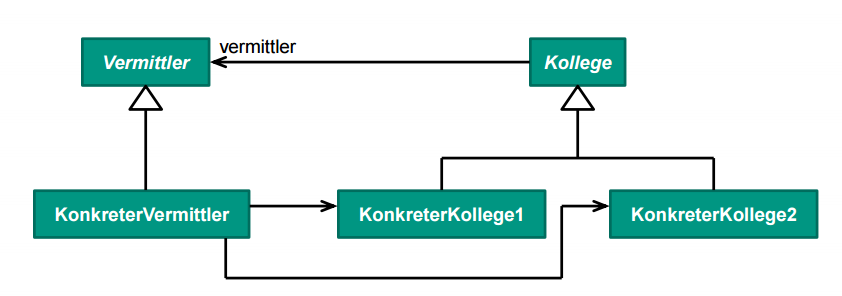
\includegraphics[scale=0.45]{./pics/tut3/med.png}
	\end{frame}

	\begin{frame}
		\frametitle{Vermittler}
		\centering
		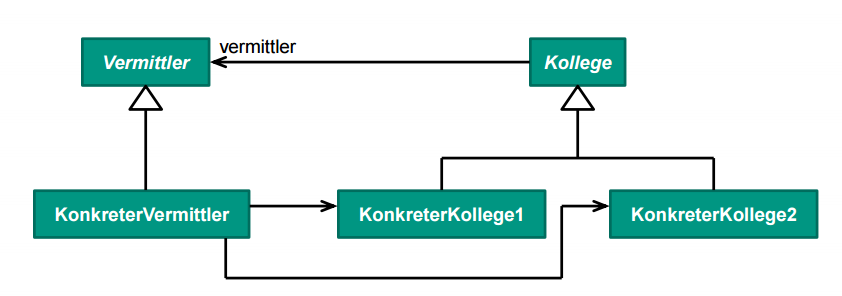
\includegraphics[scale=0.45]{./pics/tut3/med.png}
		\begin{block}{Entkopplung?}
			\begin{itemize}
				\pause 
				\item Kollegen kennen sich nicht direkt  \linebreak \pause $\implies$ Hinzufügen eines Kollegen erfordert keine Änderung der alten Kollegen
			\end{itemize}
		\end{block}
	\end{frame}

\section{Klausuraufgabe}
	\subsection{Aufgabe}
	\begin{frame}
		\frametitle{Klausuraufgabe (Hauptklausur SS 2012)}
		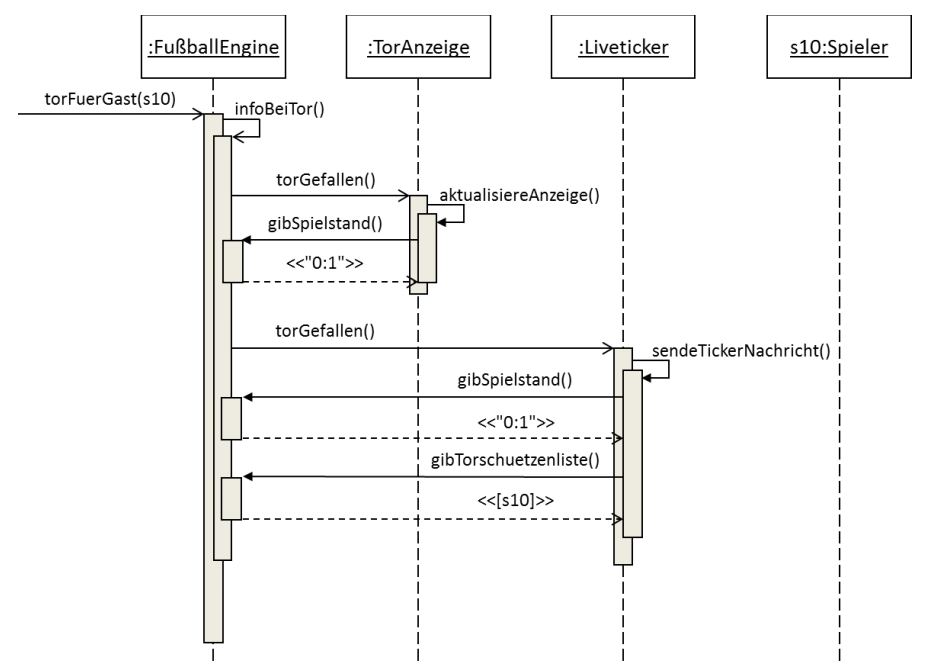
\includegraphics[scale=0.35]{./pics/tut3/obs-task.png}	
		\begin{block}{Aufgabe 1}
			Welches Entwurfsmuster erkennen Sie in diesem Diagramm? \pause
			Beobachter.
		\end{block}
	\end{frame}

	\begin{frame}
			\begin{small}
				Entwerfen Sie das folgende Klassendiagramm passend zu dem Sequenzdiagramm; es soll
				alle verwendeten Klassen und Methoden enthalten. Kennzeichnen Sie die Zugreifbarkeiten
				der Methoden mit den Symbolen +, -, \#; seien Sie dabei möglichst restriktiv. Verzichten
				Sie auf die Modellierung von Attributen. Kennzeichnen Sie die Elemente
				des Entwurfsmusters und deren Funktion.
			\end{small}
			\linebreak
			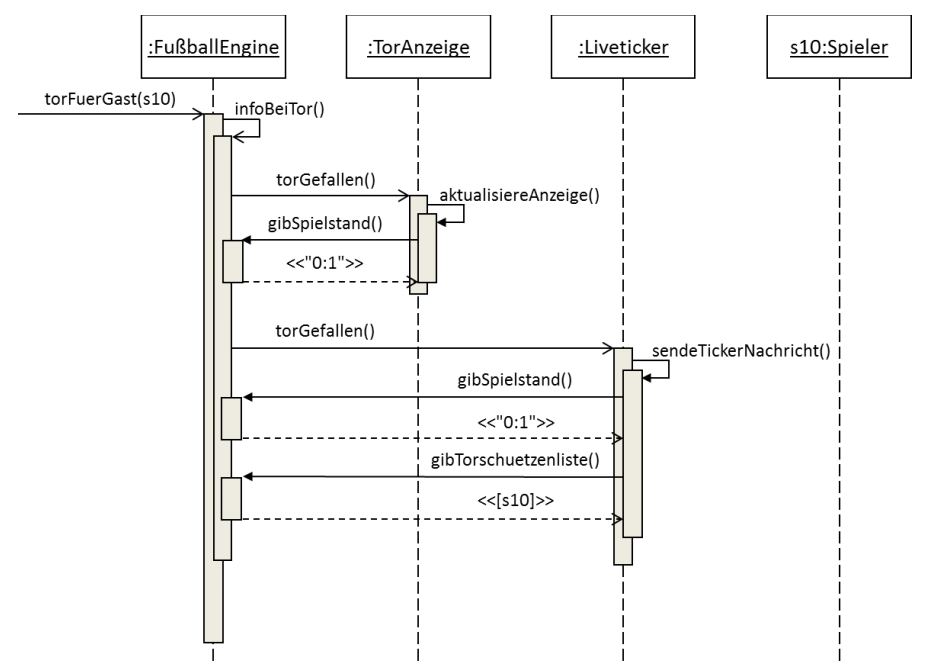
\includegraphics[scale=0.35]{./pics/tut3/obs-task.png}
	\end{frame}

	\begin{frame}
		\frametitle{Musterlösung}
		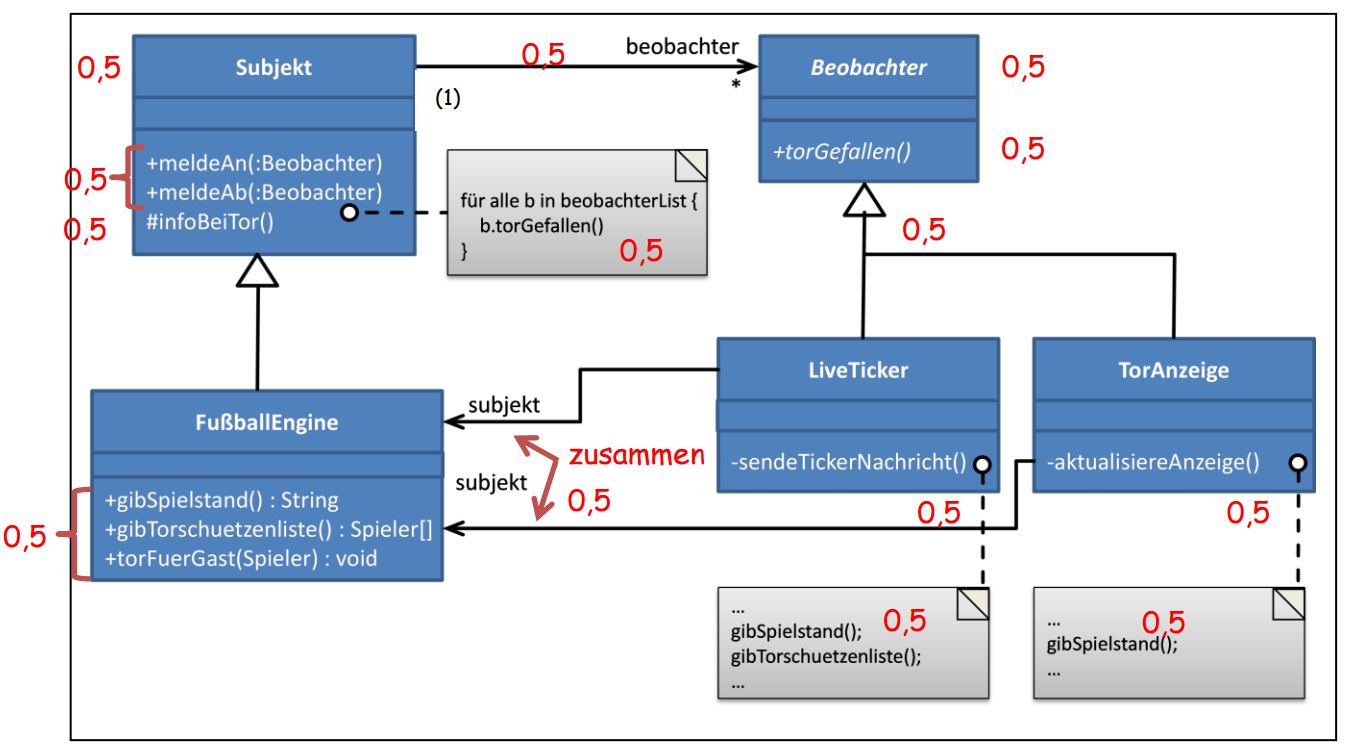
\includegraphics[scale=0.35]{./pics/tut3/obs-task-sol.png}
	\end{frame}

%TODO java swing?

\section{Tipps}
	\subsection{Tipps}
	\begin{frame}
		\frametitle{Tipps - 4. Übungsblatt}
			\begin{exampleblock}{Aufgabe 1: iMage-GUI}
				\begin{itemize}
					\item macht die "'kleinen"' Bonusaufgaben 
					\linebreak $\implies$ relativ leichte Punkte \pause
					\item schaut euch die verschiedenen LayoutManager aus Java Swing an
					\linebreak $\implies$ verschiedene LayoutManager möglich (via mehrerer Container, z.B. JPanel)
				\end{itemize}
			\end{exampleblock}
			
			\pause
			
			\begin{exampleblock}{Aufgabe 2: Zustandsdiagramm (LEZ)}
				\begin{itemize}
					\item nochmal Syntax anschauen 
					\linebreak $\implies$ Was darf in Zustandsdiagramm, was nicht? (laut VL)
					\item von Hand!
				\end{itemize}
			\end{exampleblock}
	\end{frame}

	\begin{frame}
		\frametitle{Tipps - 4. Übungsblatt}
			\begin{exampleblock}{Aufgabe 3: Git}
				\begin{itemize}
					\item echo "hallo" $>>$ test.txt schreibt hallo in test.txt
					\item git-Dokumentation anschauen
				\end{itemize}
			\end{exampleblock}
			
			\pause

			\begin{exampleblock}{Aufgabe 4: Architekturstile}
				\begin{itemize}
					\item Jmjrst (gedanklich) umbauen
					\item Zusammenhang der Klassen anschauen (z.B. Main-Klasse)
				\end{itemize}
			\end{exampleblock}
	\end{frame}
	
	\subsection{Abgabe}
	\begin{frame}
		\frametitle{Denkt dran!}
		\begin{alertblock}{Abgabe}
			\begin{itemize}
				\item Deadline am 13.6 um 12:00
				\item A2-4 handschriftlich!
			\end{itemize}
		\end{alertblock}
	\end{frame}
		
	\begin{frame}
		\frametitle{Bis dann! (dann  := 19.06.17)}
		\centering
		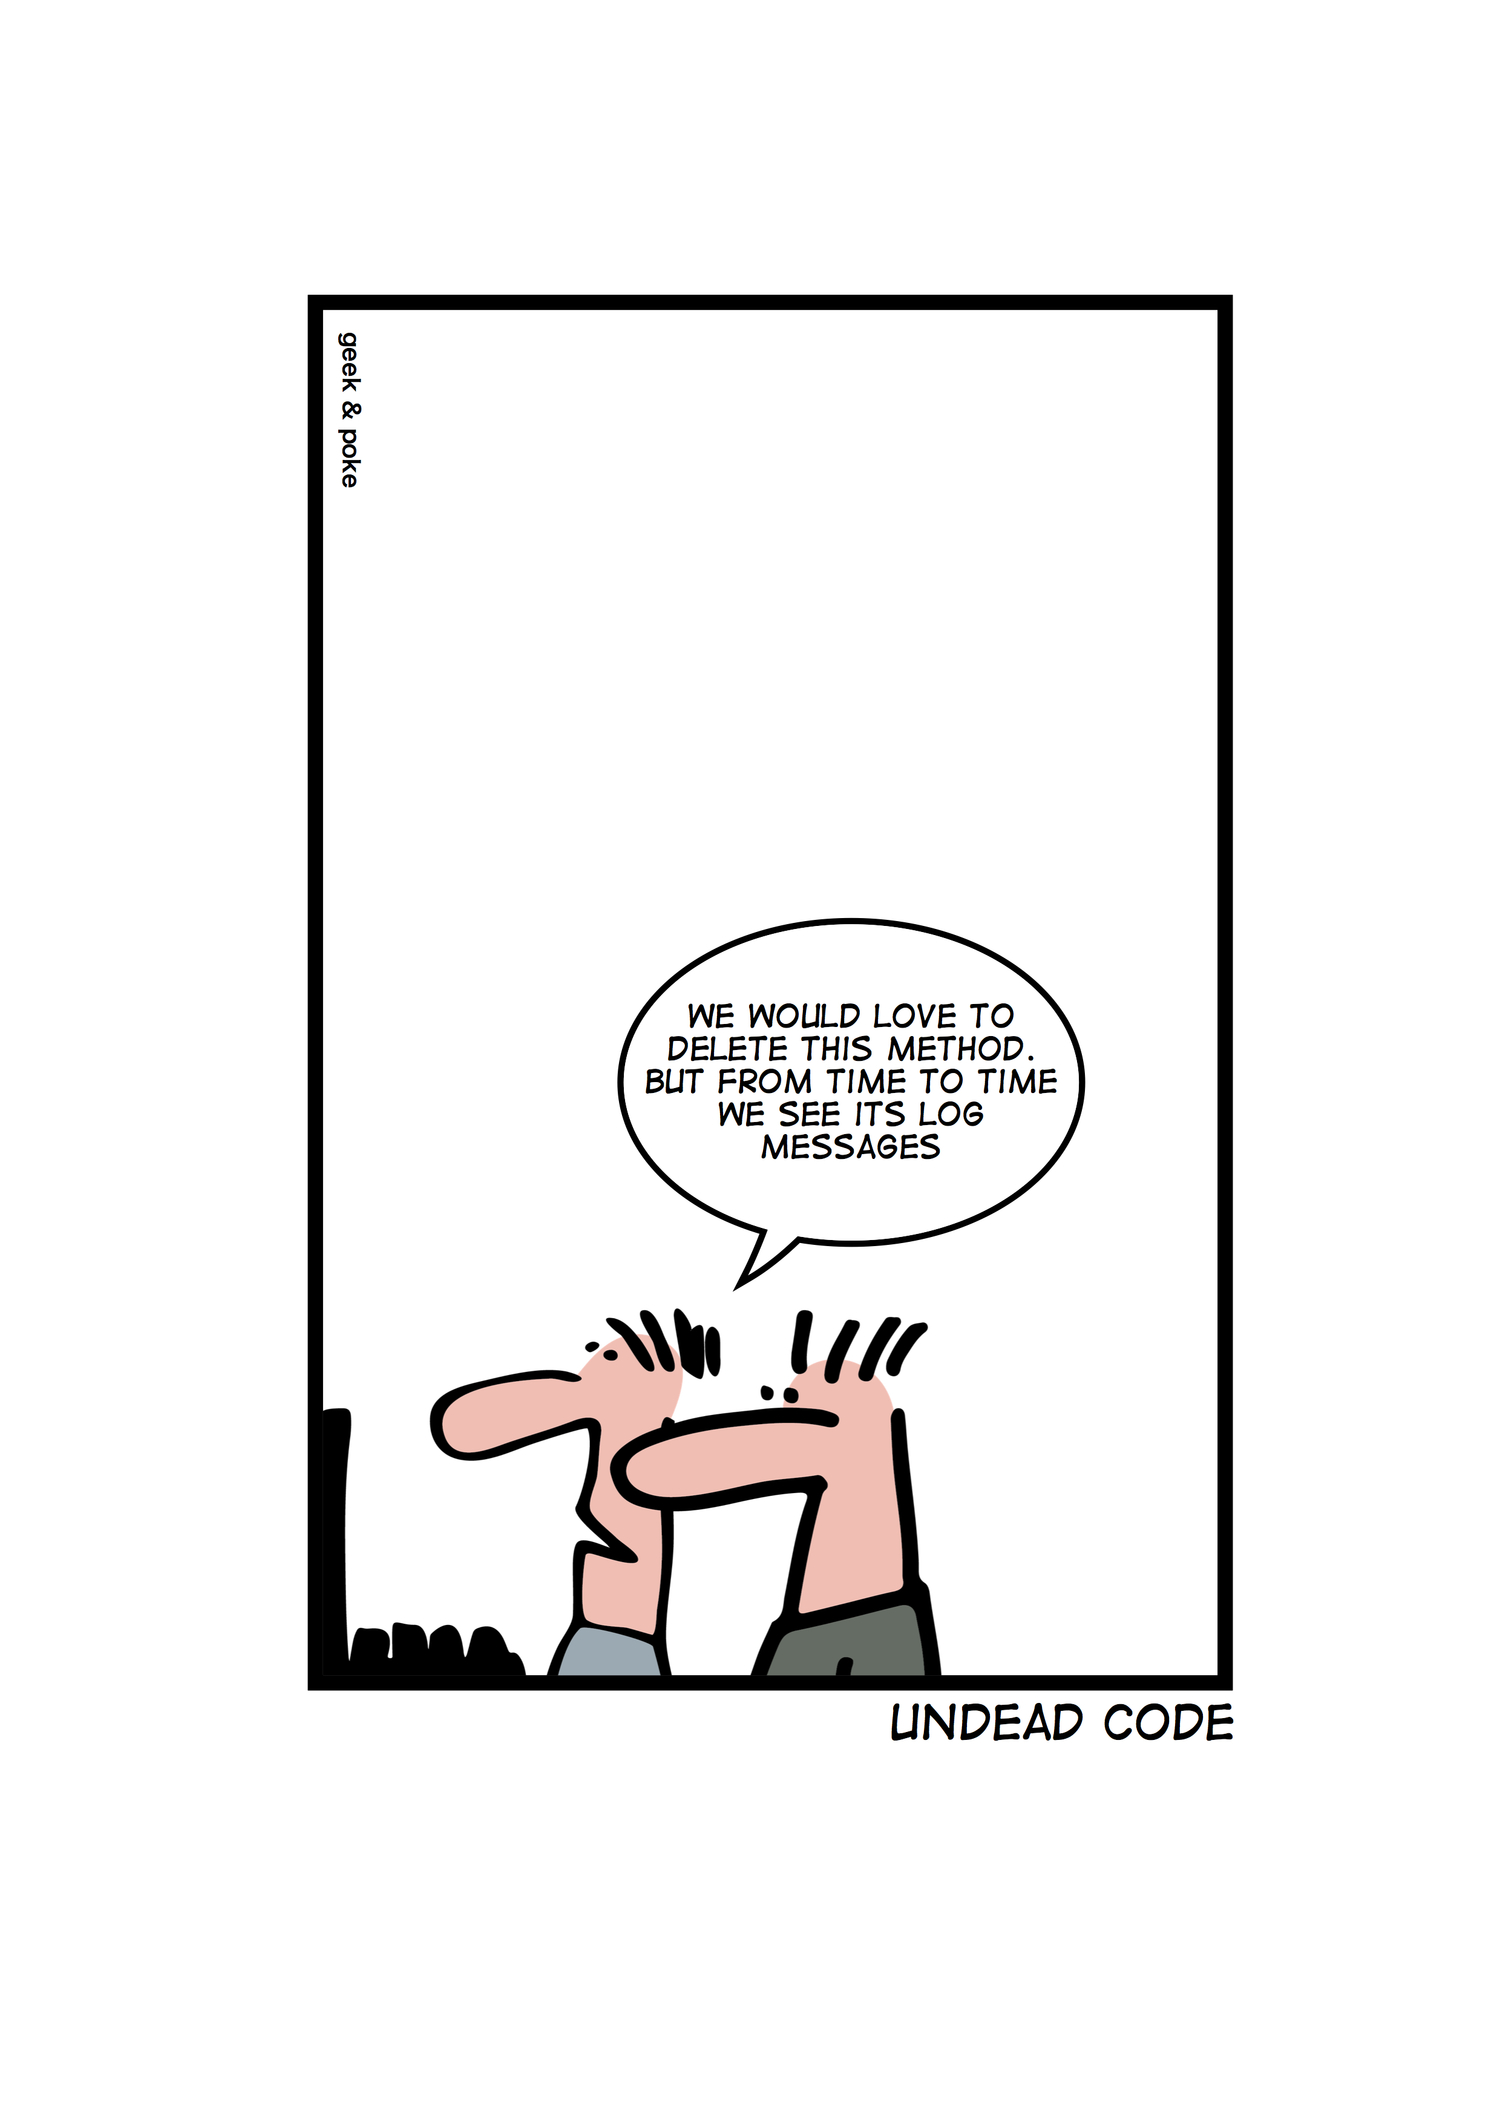
\includegraphics[scale=0.5]{./comics/geek_and_poke_undeadCode.jpg}
	\end{frame}

\end{document}